\section{Исследование и построение решения задачи}
\label{sec:Chapter3} \index{Chapter3}

Начнем исследование поставленной задачи с определения подходящих инструментов и ресурсов. Важно качественно подобрать эти элементы, чтобы их неточности не влияли на результаты экспериментов.

\subsection{Сверточная нейронная сеть}

На сегодняшний день существуют множество алгоритмов обработки лиц на изображении. Чтобы сократить список подходящих под нашу задачу алгоритмов, поставим конкретную задачу обработки. Нужно подобрать алгоритм выделения лица и построения вектора его признаков на изображении. Стоит учесть следующие факты:
\begin{enumerate}
\item Лицо занимает существенную часть изображения;
\item Лицо единственное на изображении.
\end{enumerate}
Как уже было сказано, на сегодняшний день лучшими алгоритмами построения дескриптора лица являются сверточные нейронные сети (CNN)~\cite{8,10}. Ставилась задача с помощью экспериментов определить наиболее подходящую CNN под нашу постановку. Основным критерием отбора были показатели точности поиска по евклидову расстоянию с использованием соответствующего вектора признаков. Также учитывалось время обработки изображения. В эксперименте участвовали только общедоступные CNN. Оптимальным для нашей постановки оказался алгоритм из библиотеки Python facerecognition. Во всех дальнейших исследованиях использованы дескрипторы лиц, построенные этим алгоритмом.

Здесь же стоит сказать про выбранную размерность вектора признаков. Распространенной практикой является выбор размерности равной степени двойки натурального числа. Заметим, что чем больше размерность вектора, тем больше информации о лице он может содержать, однако вектора большой размерности увеличивают как временную, так и пространственную сложность алгоритмов. Учитывая опыт связных работ, размерность дескрипторов лиц была выбрана равной 128.

\subsection{Датасет}

Выбору данных для исследования стоит уделить особое внимание. Именно от этого этапа будет зависеть применимость данного подхода на практике. Насколько выбранный датасет будет совпадать с реальными дынными, настолько можно быть уверенным в качестве полученных результатов. Снова обозначим некоторые критерии, которые будем учитывать при выборе набора данных. Во-первых, набор данных должен содержать изображения лиц. Нас будут интересовать датасеты, собранные специально для задач распознавания. Во-вторых, данных должно быть много. Мы не будем рассматривать датасеты из нескольких тысяч изображений. В-третьих, лица на фотографиях должны быть представлены в разных условиях сложности распознавания (положение, освещенность, эмоция, возраст, этническая принадлежность). Одним из самых больших датасетов лиц, подходящих под данные критерии, является VGGFace2. Изображения в нем загружаются из поиска картинок Google, что отлично подходит под исследуемую задачу. Этот набор данных содержит около 3 миллионов изображений -- фотографии более 9000 личностей, охватывающих широкий спектр разных национальностей, профессий и возрастов.

\subsection{<<Перекос>> данных}

Еще раз обратимся к Рис.~\ref{ris:multiindex}. В разбиении обычной индексной структуры можно заметить «перекос» списка кандидатов. Заметим, что эта проблема появляется и в более сложных структурах поиска. Это происходит потому, что запрос на поиск попадает близко к границе разбиения, и вследствие этого ближайший центроид не точно приближает вектор запроса. Решением данной проблемы может быть расширение списка кандидатов векторами из нескольких ближайших ячеек. Чтобы контролировать размер списка кандидатов можно добавлять соседние ячейки в рассмотрение до тех пор, пока размер списка не превысит определенного значения. Это значение подбирается экспериментально для каждой структуры.

\begin{figure}[h]
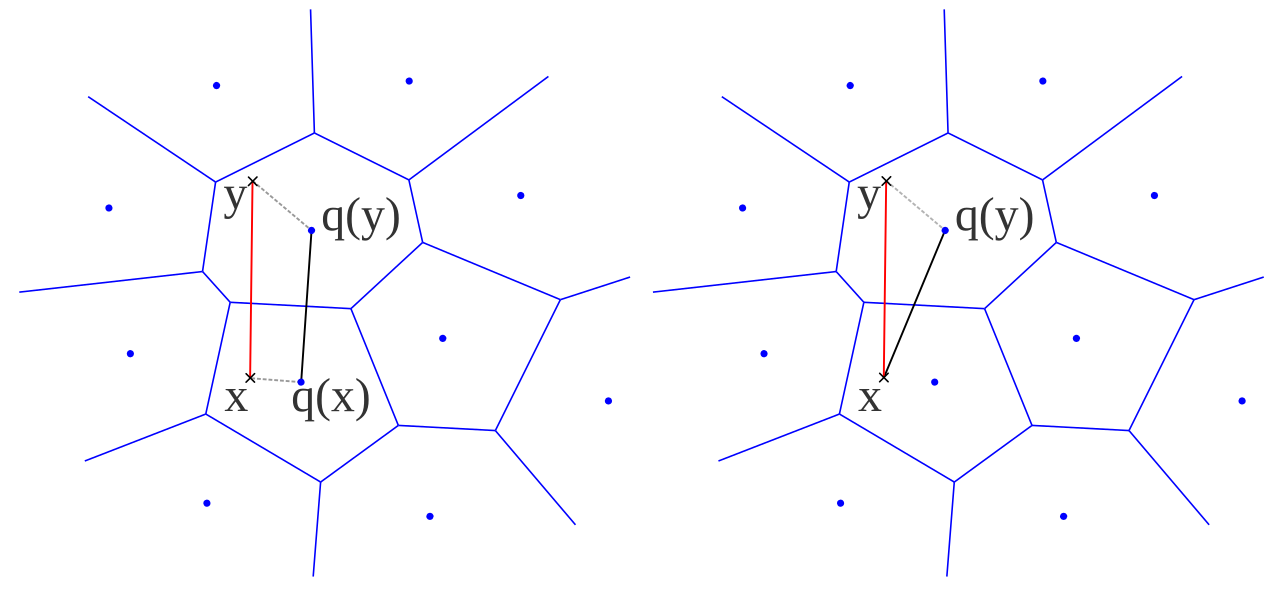
\includegraphics[width=1\linewidth]{Images/ADC_SDC.png}
\caption{Левый — симметричное расстояние. Правый — асимметричное расстояние. Расстояние $d(x,y)$ аппроксимируется расстоянием $d(q(x), q(y))$ и $d(x, q(y))$ для левого и правого рисунка соответственно.}
\label{ris:adc}
\end{figure}

\subsection{Вычисление расстояний}

Перед непосредственным описанием экспериментов опишем еще один важный момент. Рассмотрим вектор запроса $x$ и вектор индексированных данных $y$. Существует два метода вычисления приблизительного евклидова расстояния между этими векторами: симметричный и асимметричный (Рис.~\ref{ris:adc}).

Вычисление симметричного расстояния (SDC): оба вектора $x$ и $y$ представляются соответствующими центроидами $q(x)$ и $q(y)$. Расстояние $d(x, y)$ аппроксимируется расстоянием $d(x, y) = d(q(x), q(y))$, которое в случае многомерной индексации эффективно вычисляется следующим образом:
$$d(x, y) = d(q(x), q(y)) = \sqrt{\sum_{j=1}^M d(q_j(x),q_j(y))^2},$$
где расстояние между центроидами предварительно подсчитано. Справочная таблица каждого центроида содержит все квадраты расстояний до остальных центроидов.

Вычисление асимметричного расстояния (ADC): вектор $y$ представлен своим центроидом $q(y)$, а запрос $x$ не закодирован. Расстояние $d(x, y)$ аппроксимируется расстоянием $d(x, y) = d(x, q (y))$, которое вычисляется с использованием разложения:
$$d(x, y) = d(x, q(y)) = \sqrt{\sum_{j=1}^M d(x_j, q_j(y))^2)},$$
где $x_j$ — выделения компонент j-ой размерности мульти-индексного разбиения.

В обоих случаях функция корня обычно опускается. Единственное преимущество SDC перед ADC -- это меньшее использования памяти вектором запроса, поскольку он определяется своим кодом. В большинстве случаев это неактуально, поэтому используют асимметричную версию, которая позволяет получить меньшие искажения расстояния для аналогичной сложности. В остальной части работы используется ADC без явного упоминания.

\subsection{Эксперименты}

В данном разделе представлены описания экспериментов для каждой из исследуемых структур данных. Ограничимся здесь описанием основных принципов работы алгоритмов. Пошаговое описание работы каждой структуры представлено в следующем разделе.

Начнем с того, что для исследования поставленной задачи требуется огромное количество ресурсов. В связи с некоторыми ограничениями, будем проводить эксперименты на меньшем количестве данных и обобщать результат на общий случай исследования.

Для проведения экспериментов было обработано свыше 150 тысяч изображений. Для каждого из которых было произведено выделение лица и построение 128-мерного вектора признаков. Данные были сохранены в один csv-файл, который содержит информацию о 500 личностях.

Как упоминалось в постановке, нас интересует соотношения точности и скорости поиска для различных значений ближайших соседей ($K = 1, 5, 10, 30, 50, 100$). Время обучения структур не учитывается. Для чистоты экспериментов, все замеры проводятся по 1000 раз, затем результаты усредняются. На графиках ниже можно встретить две метрики точности <<Search>> и <<Recognition>>. Ломанная <<Search>> обозначает процент правильно найденных лиц среди $K$ ближайших соседей в одном запросе. Ломанная <<Recognition>> обозначает процент правильно распознанных людей во всех запросах, где успешным распознаванием считается совпадение лица запроса с лицом наибольшей частоты встречаемости среди $K$ ближайших соседей.

\subsubsection{Точный поиск}

Для сравнения результатов исследования проведем замеры точности поиска по евклидову расстоянию (Рис.~\ref{ris:euclidsearch}). Суть эксперимента в том, что данные не проходят предварительной обработки, а поиск происходит по всем имеющимся в базе данных векторам. Формируется общий ассоциативный список расстояний, который после сортировки показывает ближайшие к запросу вектора. Точность этого алгоритма будем считать эталонной, так как алгоритмы ANN не могут превысить точности исчерпывающего поиска.

\begin{figure}[h]
\begin{minipage}[h]{0.49\linewidth}
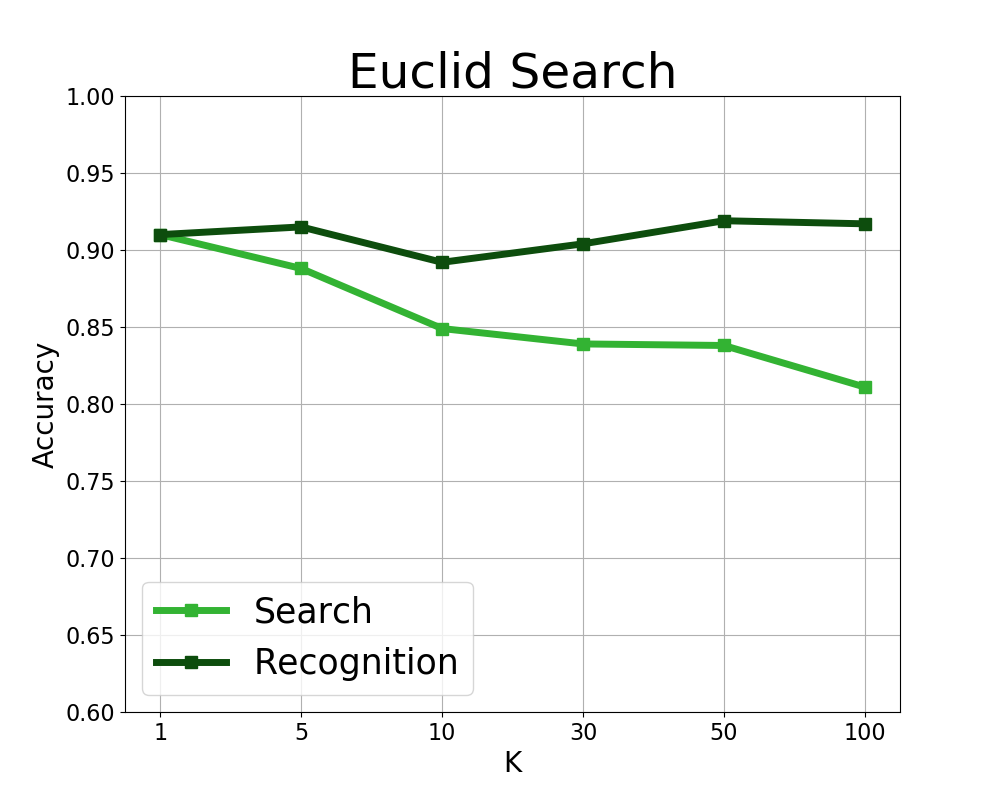
\includegraphics[width=1\linewidth]{Images/EuclidSearch.png}
\caption{Точность поиска по евклидову расстоянию.}
\label{ris:euclidsearch}
\end{minipage}
\hfill
\begin{minipage}[h]{0.49\linewidth}
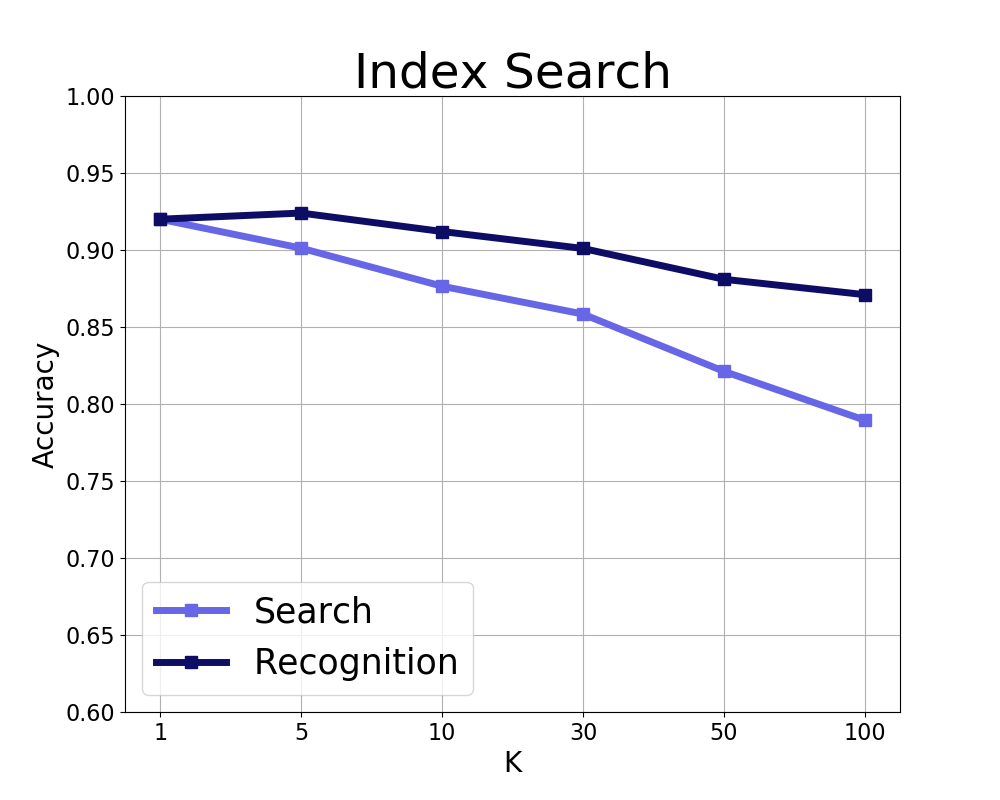
\includegraphics[width=1\linewidth]{Images/IndexSearch.png}
\caption{Точность поиска индексной структуры.}
\label{ris:indexsearch}
\end{minipage}
\end{figure}

Можно заметить и в чем мы убедимся позже, что вторая кривая находится в некоторой окрестности постоянного значения (0.90 -- 0.92). Это означает, что с расширением объема поиска процент лиц соответствующих запросу держится на одном уровне. <<Search>> кривая явно убывает, и связано это с тем, что при увеличении количества ближайших соседей вероятность попадания посторонних лиц в их число также увеличивается.

Перейдем к рассмотрению более продвинутых поисковых структур. Сначала сравним точность поиска и распознавания, а затем перейдем к оценке эффективности.

\subsubsection{Индексная структура}

Инвертированный индекс -- самый простой способ индексирования данных, но тем не менее даже он дает большой прирост в скорости поиска без ощутимого снижения качества. Для его использования требуется предобработка данных. Заметим, что из всех индексных структур, этот алгоритм требует наибольшего времени обучения, так как для построения индексной структуры используется классический алгоритм K-средних. Для исследуемых объемов данных он очень ресурсоемкий. Поиск по данной структуре разбивается на два этапа: 1) поиск ячейки; 2) поиск внутри ячейки. Для минимизации времени поиска требуется правильно подобрать параметры разбиения пространства. Путем поиска минимума функции $F(K)$ ($F(K)$ - общее количество вычислений расстояния), добиваемся оптимальной сложности поиска:
\begin{equation}\label{eq:index}
F(K)=K + \frac{N}{K},
\end{equation}
где $N$ -- объем базы данных, $K$ -- размер разбиения. 

Результаты исследования индексной структуры (Рис.~\ref{ris:indexsearch}) дают похожую картину точности, за тем лишь исключением, что общий показатель точности распознавания несколько упал (0.88 -- 0.91). Теперь при увеличении количества ближайших соседей <<Search>> кривая убывает быстрее. Это связанно с тем, что ближайшие к запросу центроиды не всегда точно определяют истинных ближайших соседей. Рассмотрение большего количества смежных ячеек улучшит результат, но негативно скажется на скорости поиска.

\begin{figure}[h]
\begin{minipage}[h]{0.49\linewidth}
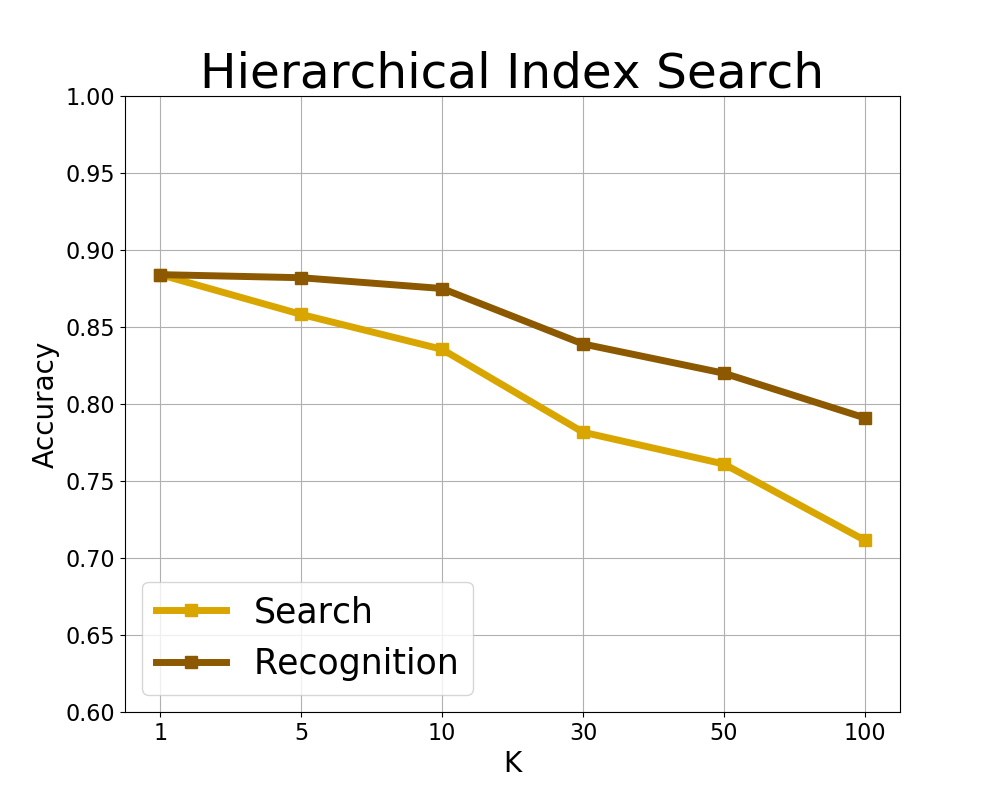
\includegraphics[width=1\linewidth]{Images/HierarchicalIndexSearch.png}
\caption{Точность поиска иерархической индексной структуры.}
\label{ris:hierarchicalindexsearch}
\end{minipage}
\hfill
\begin{minipage}[h]{0.49\linewidth}
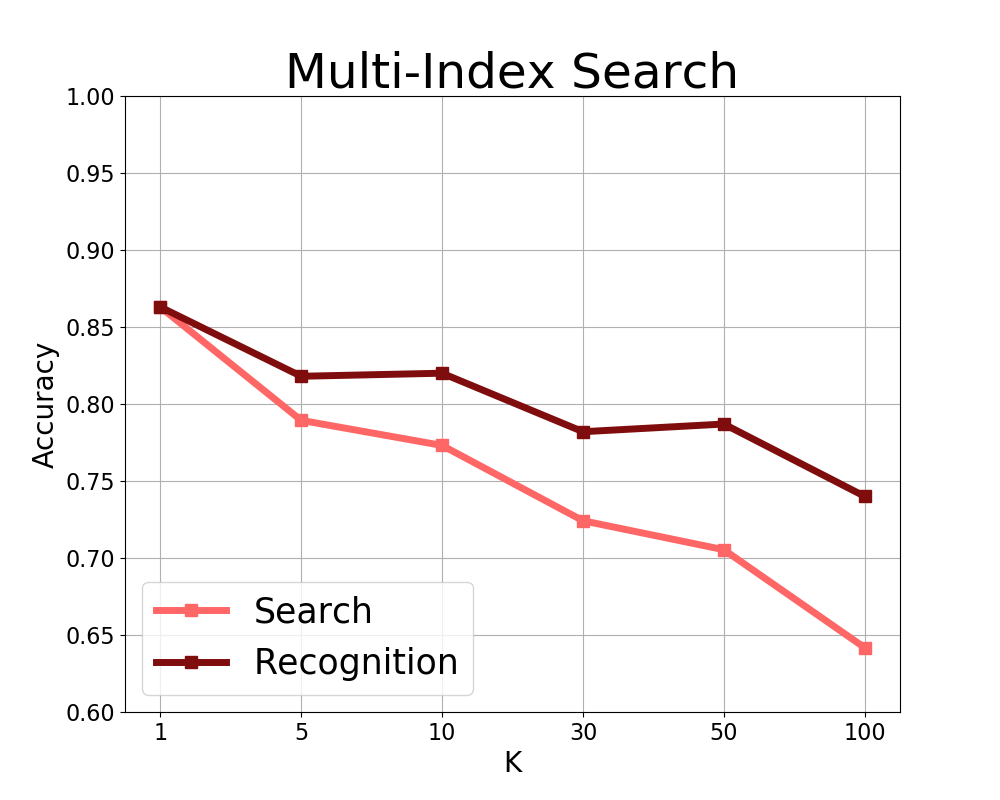
\includegraphics[width=1\linewidth]{Images/MultiIndexSearch.png}
\caption{Точность поиска мульти-индексной структуры.}
\label{ris:multiindexsearch}
\end{minipage}
\end{figure}

\subsubsection{Иерархическая структура}

Еще более существенно снизить количество вычислений помогает иерархический индекс. Этап предобрабтки для него схож с предыдущей структурой. Однако обучение происходит в несколько этапов: первичное разбиение и разбиение внутри каждой ячейки. Несмотря на большую запутанность алгоритма, обучается он на порядок быстрее. Связанно это с тем, что обучающий алгоритм существенно зависит от количества ячеек разбиения. Совокупное число ячеек здесь больше, но на каждом уровне обучения их оказывается меньше. Поиск по данной структуре тоже усложняется: 1) поиск ячейки первого уровня; 2) поиск ячейки второго уровня; 3) поиска внутри ячейки. Снова найдем минимум функции общего количества вычислений расстояния:
\begin{equation}\label{eq:hierachicalindex}
F(K_1,K_2)=K_1 + K_2 + \frac{N}{K_1K_2},
\end{equation}
где $N$ -- объем базы данных, $K_1$ и $K_2$ -- размер разбиения первого и второго уровня соответственно. 

Как видно из графика (Рис.~\ref{ris:hierarchicalindexsearch}), точность распознавания снова упала (0.82 -- 0.83). Здесь же можно заметить, что при $K = 100$ процент правильно найденных людей, среди $K$ ближайших соседей $\approx70\%$. Это ставит под вопрос применимость данной структуры в реальных задачах.

\subsubsection{Мульти-индексная структура}

Наиболее сложный и эффективный алгоритм, рассматриваемый в рамках этой работы — инвертированный мульти-индекс. Принцип его работы уже был описан в разделе <<Обзор существующих решений>>. Напомним, что этот алгоритм основан на произведении квантизации (PQ). Суть в том, что вектор разбивается на M подвекторов, и к каждому подвектору применяется классический алгоритм индексации, используя при этом отдельный список центроидов. Как было доказано в~\cite{3}, наибольшей эффективности алгоритм достигает при разбиении на два подпространства. Поэтому будем полагать, что $M = 2$. Что касается скорости обучения, то тут она еще выше. Если считать, что пространство разбивается на $K$ ячеек, то обучаться приходится лишь на $\sqrt{K}$ центроидах.

\begin{figure}[h]
\begin{minipage}[h]{0.48\linewidth}
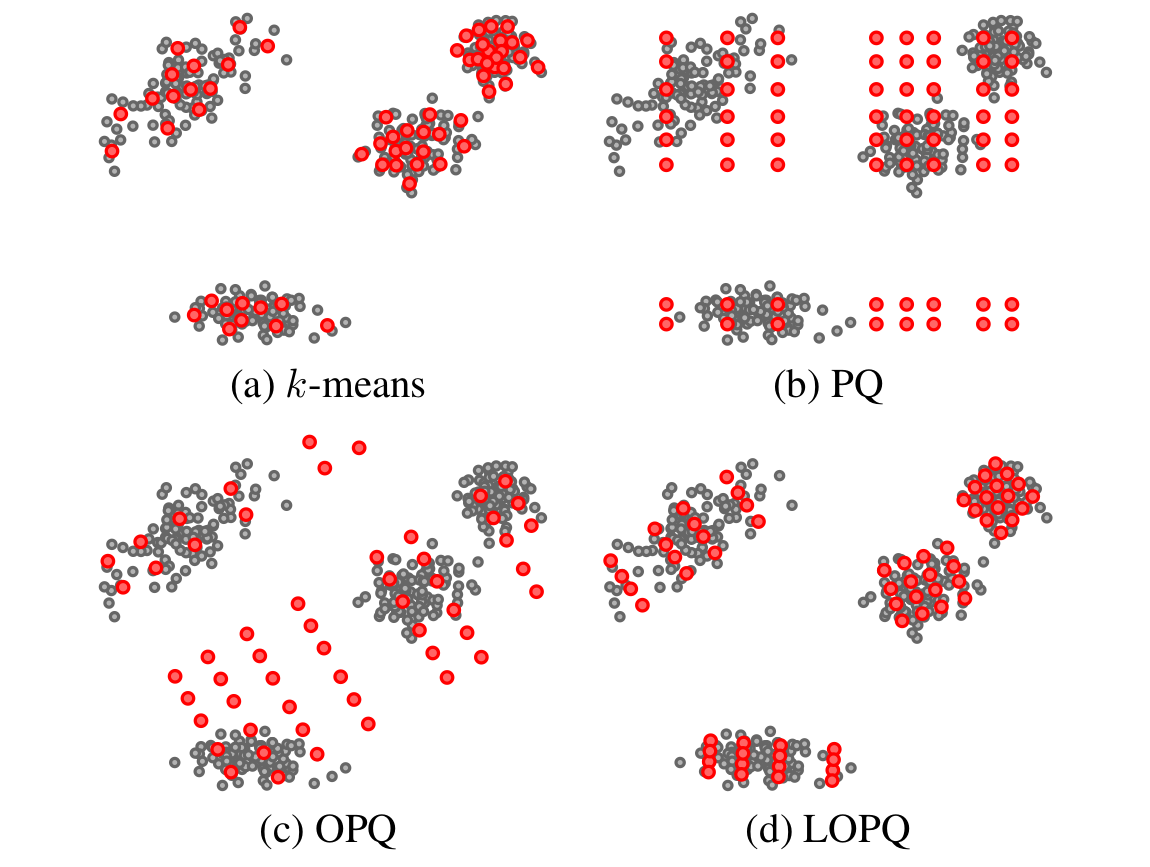
\includegraphics[width=1\linewidth]{Images/LOPQ.png}
\caption{Красными точками на рисунках обозначены центроиды. a) — инвертированный индекс; b) — инвертированный мульти-индекс; c) и d) — улeчшения мульти-индекса.}
\label{ris:lopq}
\end{minipage}
\hfill
\begin{minipage}[h]{0.48\linewidth}
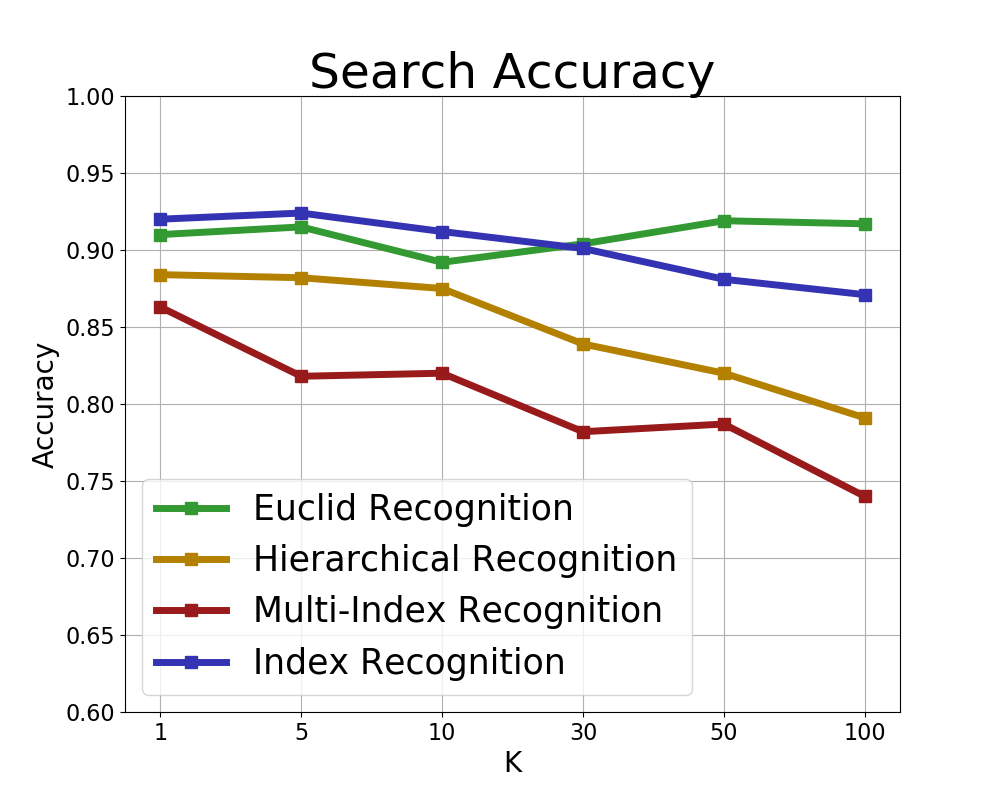
\includegraphics[width=1\linewidth]{Images/SearchAccuracy.png}
\caption{Сравнительный анализ точности поиска.}
\label{ris:searchaccuracy}
\end{minipage}
\end{figure}

Детальный алгоритм описан в следующем разделе, здесь лишь отметим, что для поиска соседей достаточно найти ближайшие центроиды всех подпространств запроса и взять их декартово произведение. Дабы снова избежать подбора параметров разбиения, найдем их оптимизацией следующей функции:
\begin{equation}\label{eq:multiindex}
F(K)= 2K + \frac{N}{K^2},
\end{equation}
где $N$ — объем базы данных, $K$ — размер разбиения каждого подпространства. 

На Рис.~\ref{ris:multiindexsearch} представлены измерения точности поиска мульти-индексной структуры. Из графика видно, что при больших значениях K показатели точности опускаются ниже $65\%$. Результат вполне очевидный, так как классическая реализация данного алгоритма показывает хороший результат только на равномерно распределенных данных, что неверно для нашего исследования. Поэтому стоит аккуратно относится к выбору этой структуры в реальных задачах.

Наглядное представление работы этих алгоритмов можно увидеть на Рис.~\ref{ris:lopq}. Здесь представлены два рассмотренных алгоритма, а также возможные пути улучшения последнего. Улучшения основаны на некоторой обработке векторов базы данных. Проблемы неравномерного распределения можно решить либо предварительным ортогональным преобразованием \cite{4,6}, либо локальными оптимизациям произведения квантизации \cite{5}.

На Рис.~\ref{ris:searchaccuracy} можно увидеть графики точности всех алгоритмов вместе. Здесь видны относительные показатели, которые позволяют сравнить алгоритмы друг с другом. Западение точности мульти-индексной структуры очевидно.

\begin{table}[h!]
\begin{tabular}{ | l | l | l | l | l | l | l | }
\hline
Алгоритм & $K = 1$ & $K = 5$ & $K = 10$ & $K = 30$ & $K = 50$ & $K = 100$  \\ \hline
Точный поиск & 0.395 & 0.339 & 0.365 & 0.347 & 0.326 & 0.343 \\
Индексная структура &0.00624 & 0.00806 & 0.00661 & 0.00687 & 0.00864 & 0.00827 \\
Мульти-индексная структура & 0.00212 & 0.00182 & 0.00211 & 0.00286 & 0.00284 & 0.00465 \\
Иерархическая структура & 0.00176 & 0.00182 & 0.00183 & 0.00151 & 0.00160 & 0.00156\\
\hline
\end{tabular}
\caption{Скорость поиска в секундах для различных значений $K$.}
\label{tab:results}
\end{table}

\begin{figure}[h]
\begin{minipage}[h]{0.49\linewidth}
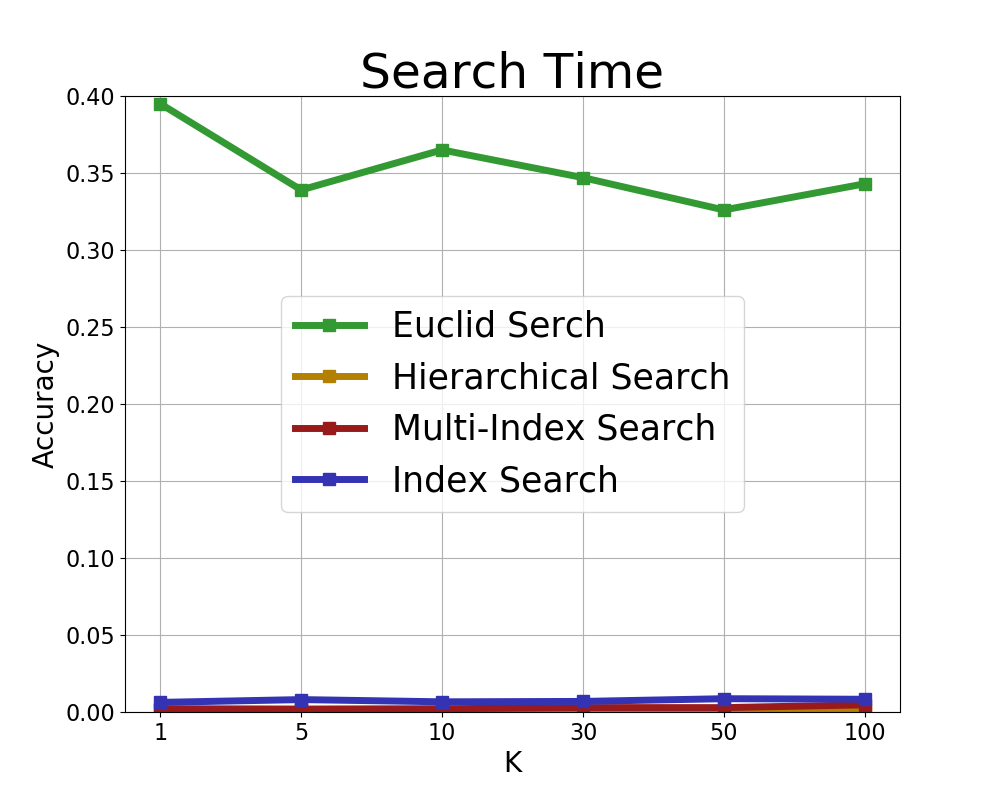
\includegraphics[width=1\linewidth]{Images/SearchTime.png}
\caption{Сравнительный анализ скорости поиска.}
\label{ris:searchtime}
\end{minipage}
\hfill
\begin{minipage}[h]{0.49\linewidth}
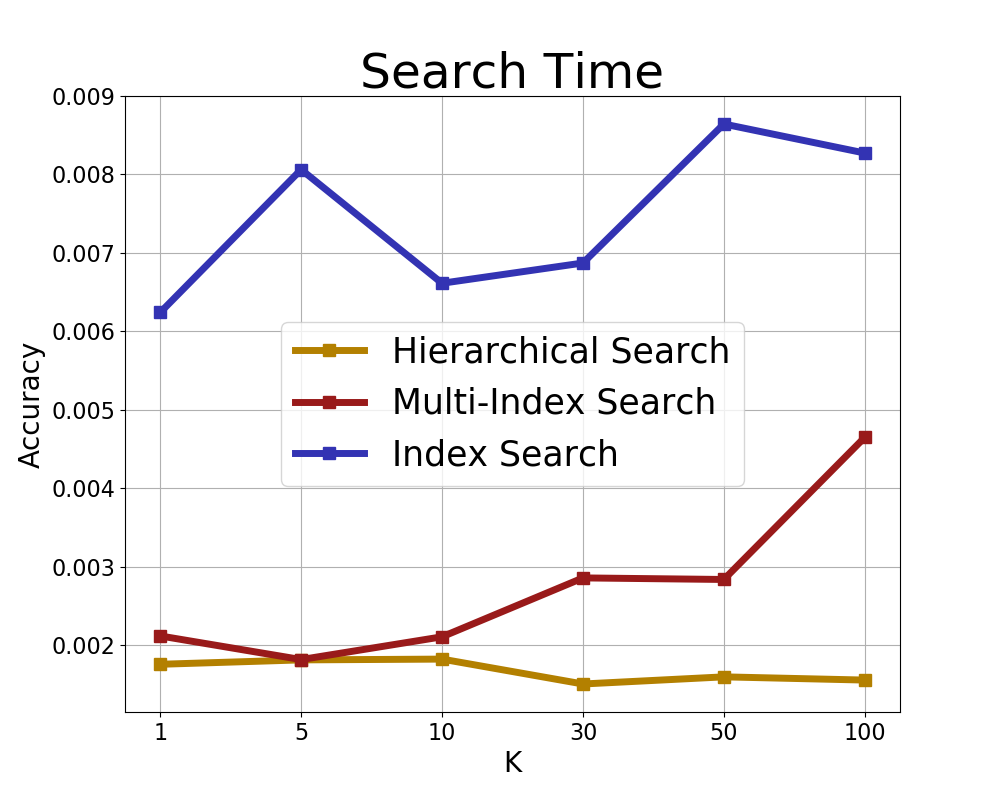
\includegraphics[width=1\linewidth]{Images/SearchTimeIndex.png}
\caption{Скорость поиска индексных структур.}
\label{ris:searchtimeindex}
\end{minipage}
\end{figure}

\subsection{Оценка времени поиска}

Теперь рассмотрим основной показатель эффективности этих структур данных. Время работы каждого запроса измерялось стандартными средствами языка программирования C++. Отсчет времени происходил с момента первого сравнения до последней сортировки кандидатов. В Таблице~\ref{tab:results} приведены численные значения результатов измерения времени. Для более наглядной оценки результатов приведен график зависимости времени поиска от $K$ (количество ближайших соседей) (Рис.~\ref{ris:searchtime}). Легко заметить, что любая индексная структура ускоряет поиск в сотни раз по сравнению с исчерпывающим поиском. На Рис.~\ref{ris:searchtimeindex} изображены ломанные соответствующие времени поиска только индексных структур для различных значений K ближайших соседей. Основная тенденция ломанных идет на возрастание, что связанно с тем, что при увеличении количества ближайших соседей также увеличивается список кандидатов. Резкие скачки на графике объясняются опять же неравномерностью распределения данных.